
\bbbbb{Illustrations of Pipeline Phenomena}%
 \label{Illustrations of Pipeline Phenomena}

\begin{figure}[ht]
  \begin{center}
  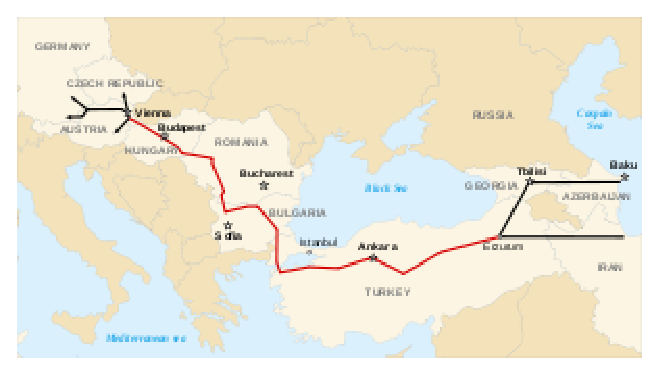
\epsfig{file=Nabucco.eps,height=\pos{4.5}{9}cm}
  \end{center}
    \caption{\brcolor{The Planned Nabucco Pipeline:}
    \pos{http://en.wikipedia.org/wiki/Nabucco\_Pipeline}{}}\label{pl.dia2} 
\end{figure}


\noindent
\begynd
\pind The Nabucco pipeline was, for many years, a planned pipeline
involving Austria, Turkey, Iran and other states and companies.
\afslut

\mnewfoil

\begin{figure}[ht]
  \begin{center}
  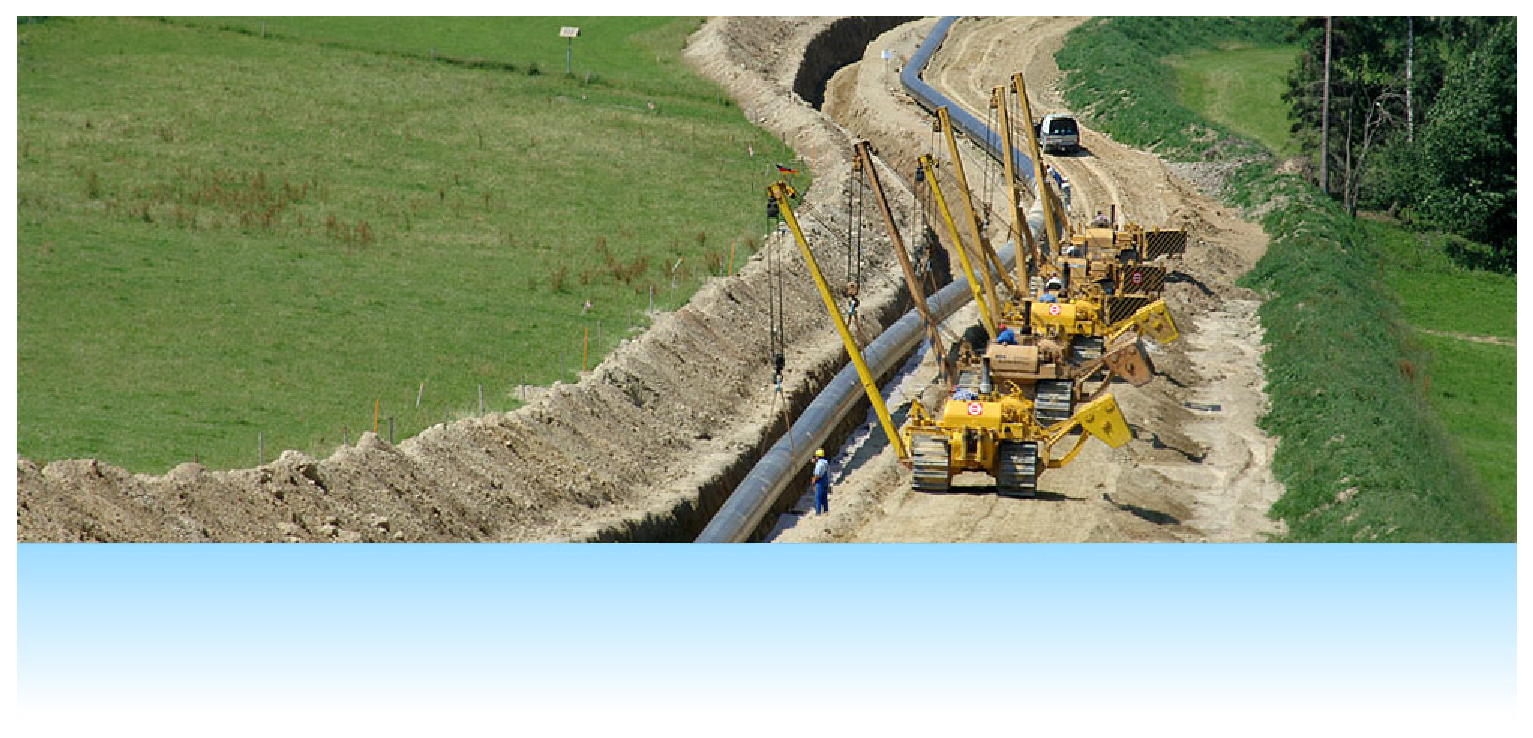
\epsfig{file=nabucco-digging,height=\pos{3.85}{11}cm}
  \end{center}
    \caption{\brcolor{Pipeline Construction}}\label{pl.dia3}
\end{figure}

\noindent
\begynd
\pind An example pipeline construction.
\pind It shows the linking of pipe segments.
\afslut
%\mnewfoil


\nbbbb{Pipes}

\begin{figure}[ht]
  \begin{center}
 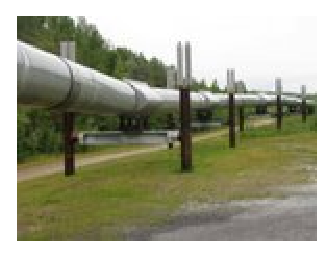
\epsfig{file=pipeline-1.eps,height=\pos{3.4}{6}cm}\ \ 
 
\epsfig{file=pipeline-2.eps,height=\pos{3.4}{6}cm}\ \ 
 
\epsfig{file=pipeline-3.eps,height=\pos{3.4}{6}cm}
  \end{center}
    \caption{\brcolor{Pipe Segments}}\label{pl.pipes}
 \end{figure}

\noindent
\begynd
\pind A pipe segment is a straight ``tube''-like unit.
\afslut
\nbbbb{Valves}
 
\begin{figure}[ht]
  \begin{center}
  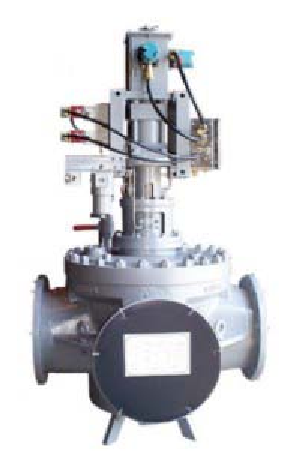
\epsfig{file=4Way-valve.eps,height=\pos{3.4}{6}cm}\ \ 
  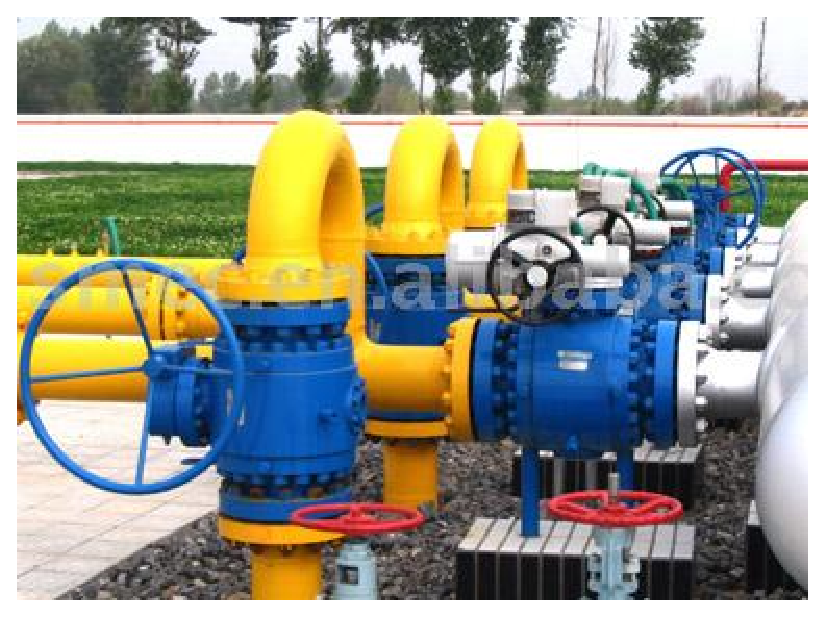
\epsfig{file=ball-valves.eps,height=\pos{3.4}{6}cm}\ \ 
  
\epsfig{file=butterfly-valve-1.eps,height=\pos{3.4}{6}cm}\ \ 
  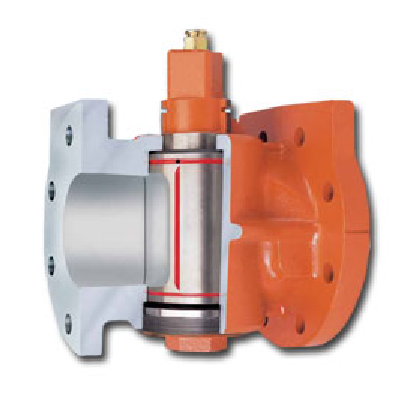
\epsfig{file=Resun-Plug-Valve.eps,height=\pos{3.4}{6}cm}
  \end{center}
    \caption{\brcolor{Valves}}\label{pl.valves}
 \end{figure}

\noindent
\begynd
\pind A pipe valve allows for the control of flow in pipes.
\afslut

\nbbbb{Pumps}
 
\begin{figure}[h]
  \begin{center}
      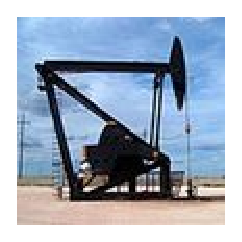
\epsfig{file=oil-drain-pump.eps,height=\pos{3.5}{7}cm}\ \ \ \ \
      \ \ \ \
      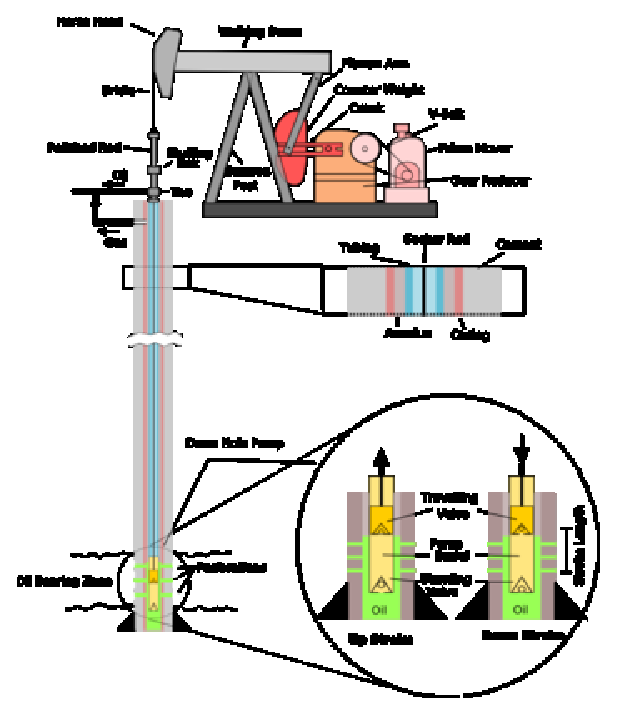
\epsfig{file=pump-jack.eps,height=\pos{3.5}{7}cm}
  \end{center}
    \caption{\brcolor{Oil Pumps}}\label{pl.pumps}
 \end{figure}

\noindent
\begynd
\pind A pump allows for the ``lifting'' of, for example, oil, over
      hilly terrain.
\pind The concept of \sfsl{pump head [height]} is relevant:
\begynd
\pind The \sfsl{head} is the height at which a pump can raise fluid up
      \nyl and is measured in meters or feet.
\afslut
\afslut

\nbbbb{Compressors}
 
\begin{figure}[h]
  \begin{center}
      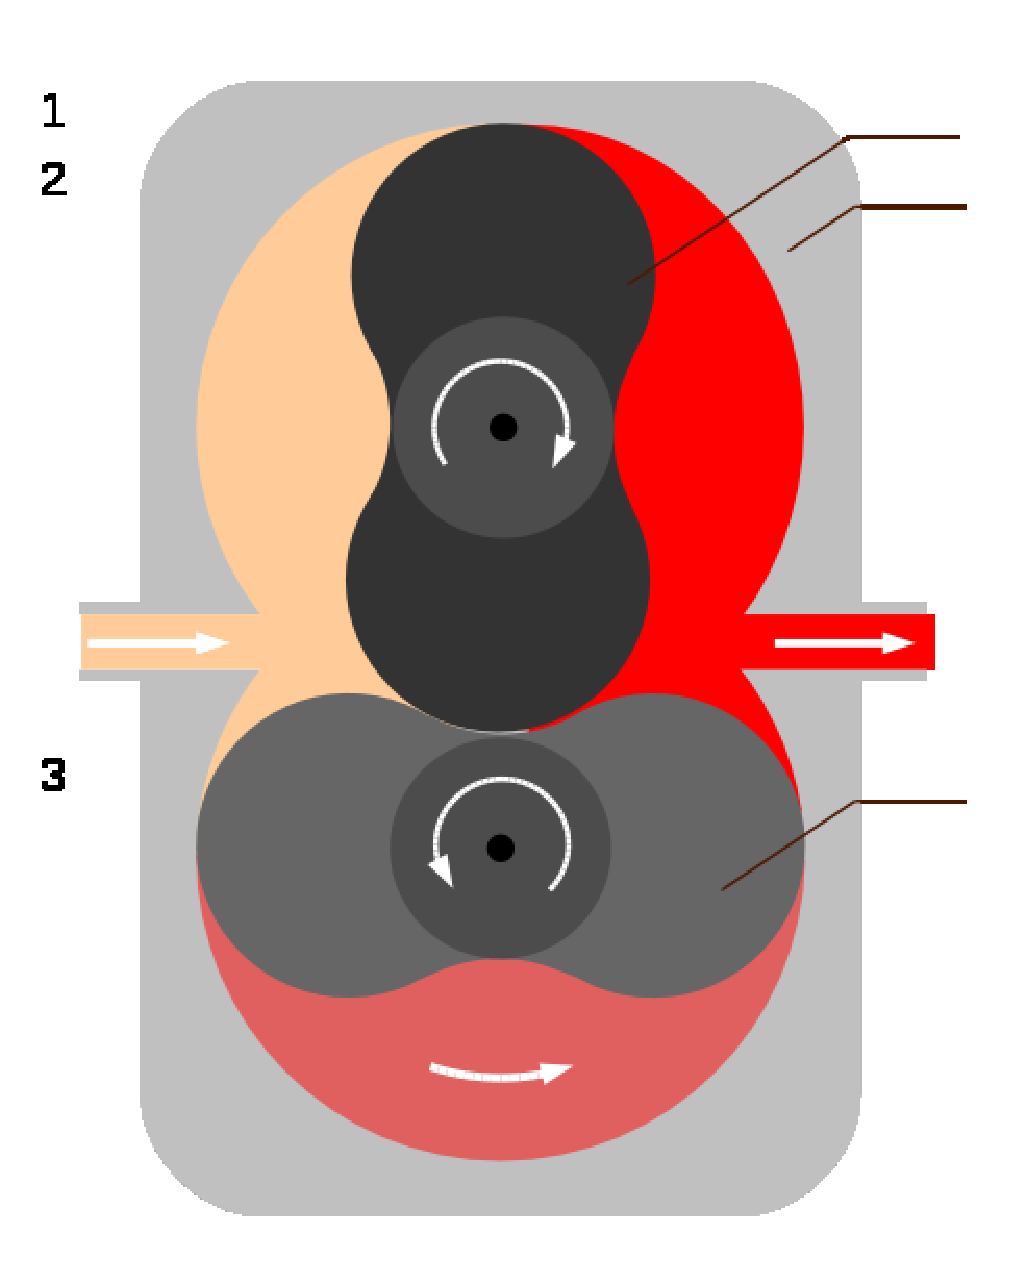
\epsfig{file=rotary-piston-pump.eps,height=\pos{3.4}{7}cm}\ \ \ 
      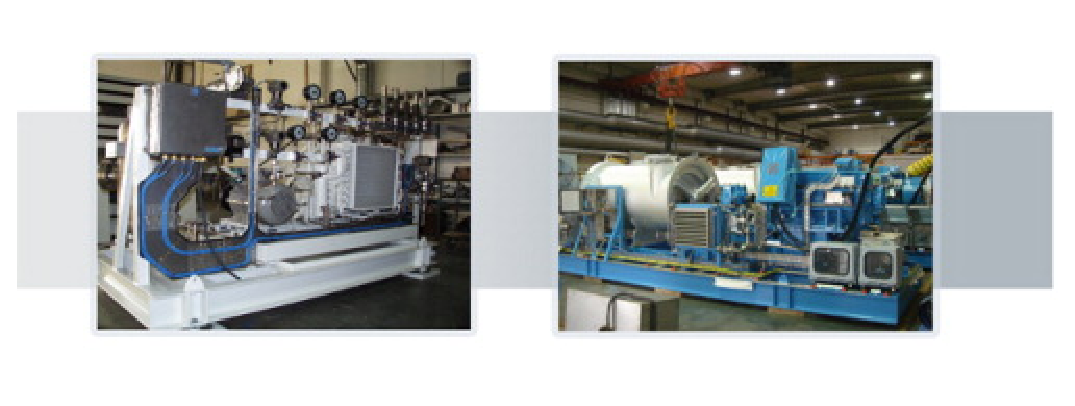
\epsfig{file=gas-compressor.eps,height=\pos{3.4}{7}cm}
  \end{center}
    \caption{\brcolor{Gas Compressors}}\label{pl.compressors}
 \end{figure}

\noindent
\begynd
\pind A compressor is used for gaseous liquids.
\begynd
\pind Compressors are similar to pumps: \nyl both increase the pressure on a fluid \nyl and both can transport the fluid through a pipe. \nyl As gases are compressible, \nyl the compressor also reduces the volume of a gas. 
\afslut
\afslut

\nbbbb{Pigs}
 
\begin{figure}[h]
  \begin{center}
  
\epsfig{file=pig.eps,height=\pos{3.4}{7}cm}\ \ \ 
  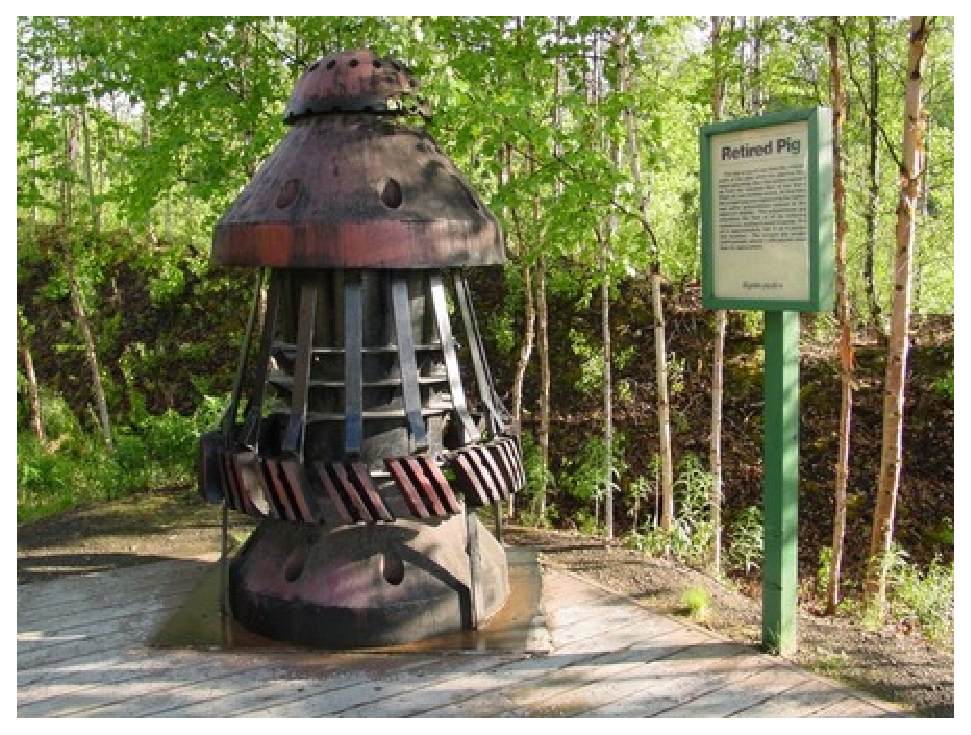
\epsfig{file=retired-pig.eps,height=\pos{3.4}{7}cm}
  \end{center}
    \caption{\brcolor{New and Old Pigs}}\label{pl.pig2} 
\end{figure}

\noindent
\begynd
\pind A ``pig'' is a tool that is sent down a pipeline and propelled
by the pressure of the product flow in the pipeline itself.  
\pind The primary purpose of pipeline pigs is to make sure that the
pipe is clean and free from obstruction.  
\afslut
\mnewfoil

\begin{figure}[h]
  \begin{center}
  
\epsfig{file=GasPigTrap.eps,height=\pos{3.4}{7}cm} \ \ 
  
\epsfig{file=pig-receivers.eps,height=\pos{3.4}{7}cm}
  \end{center}
    \caption{\brcolor{Pig Launcher, Receiver}}\label{pl.pig1} 
 \end{figure}

\mnewfoil

\begin{figure}[ht]
  \begin{center}
    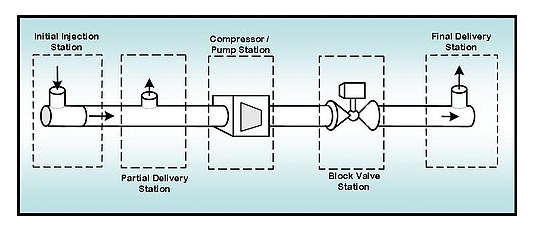
\epsfig{file=pipeline-diagram.eps,height=\pos{5}{8}cm}
    \caption{\brcolor{A Simple Pipeline}}\label{pi:pl.dia0}
  \end{center}
 \end{figure}

\noindent
\begynd
\pind Leftmost: A \sort{Well}. 
\pind 2nd from  left: a \sort{Fork}.
\pind Rightmost: a \sort{Sink}.
\afslut  
\mnewfoil

\begin{figure}[ht]
  \begin{center}
   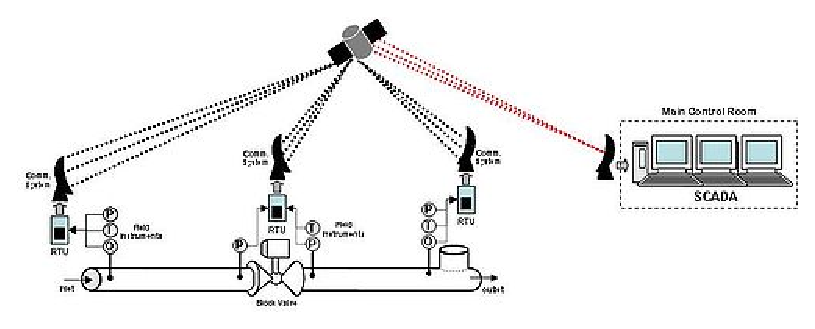
\epsfig{file=pipeline-scada.eps,height=\pos{5}{8}cm}
  \end{center}
    \caption{\brcolor{\LLLL\HHHH A Pipeline Monitoring \& Control System Diagram}}\label{pi:pl.dia1}
 \end{figure}

\noindent
\begynd
\pind Also called \sfsl{SCADA [Supervisory Control And Data Acquisition]}
\afslut 
%%  LocalWords:  Nabucco nd SCADA
